\documentclass[10pt]{article}

\usepackage[utf8]{inputenc}

\usepackage{graphicx} % for figures
\usepackage{ccaption} % captions on different pages

%% BASED ON TEMPLATE GIVEN FOR PLOS

% amsmath package, useful for mathematical formulas
\usepackage{amsmath}
% amssymb package, useful for mathematical symbols
\usepackage{amssymb}

% cite package, to clean up citations in the main text. Do not remove.
\usepackage{cite}

\usepackage{hyperref}

% line numbers
\usepackage{lineno}

% ligatures disabled
\usepackage{microtype}
\DisableLigatures[f]{encoding = *, family = * }

% rotating package for sideways tables
%\usepackage{rotating}

% If you wish to include algorithms, please use one of the packages below. Also, please see the algorithm section of our LaTeX guidelines (http://www.plosone.org/static/latexGuidelines) for important information about required formatting.
%\usepackage{algorithmic}
%\usepackage{algorithmicx}

% Use doublespacing - comment out for single spacing
%\usepackage{setspace} 
%\doublespacing


% Text layout
\topmargin 0.0cm
\oddsidemargin 0.5cm
\evensidemargin 0.5cm
\textwidth 16cm 
\textheight 21cm

% Bold the 'Figure #' in the caption and separate it with a period
% Captions will be left justified
\usepackage[labelfont=bf,labelsep=period,justification=raggedright]{caption}

% Use the PLoS provided BiBTeX style
%\bibliographystyle{plos2009} % NOW in drosprpaper.tex

% Remove brackets from numbering in List of References
\makeatletter
\renewcommand{\@biblabel}[1]{\quad#1.}
\makeatother


% Leave date blank
\date{}

\pagestyle{myheadings}

%% Include all macros below. Please limit the use of macros.

%% END MACROS SECTION

%%% MY STUFF %%%

% my packages

\usepackage{gensymb}
\usepackage{setspace} % for 1.5 spacing
\usepackage{verbatim} % multiline comments
\usepackage{acronym}

\usepackage{rotating} % sidewaysfigure

\acrodef{RF}{receptive field}
\acrodef{RIDF}{rotational image difference function}
\acrodef{rms}[r.m.s.]{root mean square}
\acrodef{ANN}{artificial neural network}

%\usepackage{todonotes}
%\usepackage{soul}
%%\newcommand{\hltodo}[2]{\texthl{#1}\todo{#2}}
%\newcommand{\hltodo}{}
%\usepackage{pdfcomment}

% header stuff
\usepackage{fancyhdr}
\setlength{\headheight}{15.2pt}
\pagestyle{fancy}

\newcommand{\Matlab}{MATLAB}

%\newcommand{\thesiscontcaption}[1]{\caption[#1]{#1 (Continued on next page.)}}

\begin{document}

%\newcommand{\draft}{D8} %% NOW IN drosprpaper.tex

\begin{comment}
\lhead{\today}
\chead{Draft: \draft}
\rhead{Section: \thesection}
\end{comment}

\doublespacing


\newcommand{\citeA}[1]{\cite{#1}}
\newcommand{\draft}{tex}

% Title must be 150 characters or less
\begin{flushleft}
{\Large
\textbf{Neural coding in \emph{Drosophila}: What visual tasks can be underpinned by small population codes}
}
% Insert Author names, affiliations and corresponding author email.
\\
Alex D. M. Dewar$^{1}$,
Antoine Wystrach$^{2}$,
Andrew Philippides$^{3}$,
Paul Graham$^{1,\ast}$
\\
\bf{1} Alex D. M. Dewar and Paul Graham, School of Life Sciences, John Maynard Smith Building, University of Sussex, Falmer, BN1 9QJ, UK.
\\
\bf{2} Antoine Wystrach, School of Informatics, University of Edinburgh, Appleton Tower, 11 Crichton Street, Edinburgh, EH8 9LE, UK.
\\
\bf{3} Andrew Philippides, Department of Informatics, Chichester I, University of Sussex, Falmer, Brighton BN1 9QJ, UK.
\\
$\ast$ E-mail: paulgr@sussex.ac.uk
\end{flushleft}

\section*{Abstract}
All organisms wishing to survive and reproduce must be able to respond adaptively to a complex, changing world.
Yet the computational power available is constrained by biology and evolution, thus favouring mechanisms that are parsimonious yet robust.
Here we show the power given by a small number of visually responsive neurons in \emph{Drosophila melanogaster} for solving complex behavioural tasks including pattern recognition.
Our findings indicate that flies' performance on some tasks may be better understood by taking a bottom-up approach and looking at the combined activity of general processing mechanisms, rather than as the product of more specialised cognitive modules.


\section{Introduction}
% [PRG]
% incorporating andy's comments 26/09/15

As with many animals, vision plays a key role in a number of behaviours performed by the fruitfly \emph{Drosophila melanogaster}, including mate-recognition \cite{Agrawal2014}, place homing \cite{Ofstad2011}, visual course control \cite{Borst2014}, collision-avoidance \cite{Tammero2002}, landing \cite{Tammero2002} and escaping a looming object (like a rolled newspaper, for example) \cite{Card2008}. The benefit of studying these visually guided behaviours in \emph{Drosophila} is, of course, the range of neurogenetic techniques which give a realistic chance of understanding the neural circuits that underpin them. With that goal in mind, we focus on recent work \cite{Seelig2013} which has mapped the receptive fields of a set of visually responsive neurons, the ring neurons of the ellipsoid body, which are surprisingly small in number given that they are key for certain complex behaviours \cite<e.g.,>{Liu2006,Neuser2008,Seelig2015}. To understand their behavioural role, it is desirable to investigate the response of these cells during experiments designed to elucidate these behaviours. In this chapter, we use modelling to bridge the gap between neurogenetic data and behaviour by evaluating neural responses during simulated behaviour. In this way we investigate how small populations of well-described visual neurons in \emph{Drosophila} provide behaviourally relevant information.

In laboratory assays flies show interesting spontaneous visual behaviours. For instance, flies will orient towards bar stimuli \cite{Reichardt1969,Gotz1987} and in a circular arena with two diametrically placed bars will walk between them for long periods. This spontaneous preference for elongated vertical bars is reduced as the bar is shortened until free-flying flies show a spontaneous aversion to small cube stimuli \cite{Maimon2008}. In addition to a suite of visual reflexes, \emph{Drosophila} also demonstrate complex visual behaviours involving interactions between orientation and memory.
For instance, a number of papers have investigated the process of pattern recognition and its neural underpinnings \cite{Ernst1999,Liu2006,Pan2009}.
The standard paradigm involves putting a fly into a closed-loop system where it is tethered in a drum, on the inside of which are two visual stimuli alternating every 90\degree\ (Figure~\ref{fig:drosopattern:recap}E). As the fly attempts to rotate in one direction, the drum counter rotates, giving the illusion of closed-loop control. To elicit conditioned behaviour, if the fly faces one of the patterns it receives negative reinforcement, a heat beam or laser which heats the abdomen. Over time if the fly is able to differentiate the patterns it will preferentially face the unpunished pattern. This procedure has been used to demonstrate that flies can differentiate stimulus pairs such as upright and inverted `T' shapes, a small and a large square, and many others \cite{Ernst1999}. That is, flies seem to possess a form of pattern recognition and pattern memory analogous to the better studied pattern memory of bees \cite{vonFrisch1914,Giurfa1997,Horridge2009}.

Here we re-examine these experiments by simulating the visual input as it would be processed through newly mapped visually responsive cells. The control of these visual behaviours is dependent on the central complex of flies, a brain area thought to be involved primarily in spatial representation and mediation between visual input and motor output \cite{Pfeiffer2014}.
The central complex comprises the ellipsoid body, the fan-shaped body, the paired noduli and the protocerebral bridge \cite{Young2010}.
This part of the brain has been characterised as the site of action selection and organisation and is claimed to be homologous to the basal ganglia in vertebrates \cite{Strausfeld2013}.
In the ellipsoid body, there are a class of neurons called `ring neurons', which are known to be involved in visual behaviours (R1: place homing \cite{Sitaraman2008,Sitaraman2010,Ofstad2011}; R2/R4m: pattern recognition \cite{Ernst1999,Liu2006,Pan2009}; R3/R4: bar fixation memory \cite{Neuser2008}).

Beyond the identification of brain regions associated with specific behaviours it is now possible to describe the properties of specific visual cells in the central complex. \citeA{Seelig2013} have studied two classes of ring neuron in the \emph{Drosophila} ellipsoid body.
The two subtypes of ring neuron investigated were the R2 and R4d ring neurons, of which only 28 and 14, respectively, were responsive to visual stimuli.
The cells were found to possess \acp{RF} that were large, centred in the ipsilateral portion of the visual field and with forms similar to those of mammalian simple cells \cite{Hubel1962} (for details of how the receptive fields were estimated, see Section~\ref{sec:drosopattern:methods:seelig}).
Like simple cells, many of these neurons showed strong orientation tuning and some were directionally sensitive.
The ring neuron \acp{RF}, however, are much coarser in form than simple cells, are far larger, are less evenly distributed across the visual field and respond mainly to orientations near the vertical.
This suggests that ring neurons might have a less general function than simple cells \cite{Wystrach2014CB}.
The population of simple cells means that small high contrast boundaries of any orientation are detected at all points in the visual field.
Thus the encoding provided by simple cells preserves visual information about bars and edges that could be used as a `general-purpose' network feeding into any number of behaviours.
In contrast, the coarseness of the receptive fields of ring neurons, allied to the tight relationship between specific behaviours and sub-populations of ring neurons suggests instead that these cells are providing economical visual information in a behaviourally tuned way.

To investigate such issues, we here advocate the use of a synthetic approach whereby investigations, in simulation, of the information provided by these populations of neurons can be related to behavioural requirements, thus `closing the loop' between brain and behaviour. We show how the population code is well-suited to the spontaneous bar orientation behaviours shown by flies. Similarly, we verify that our population of simulated ring neurons are able to discriminate visual patterns to the same standard as flies.
Upon deeper analysis, we demonstrate that certain shape parameters -- orientation, size and position -- are implicit in the ring neurons' outputs to a high accuracy, thus providing the information required for a suite of basic fly behaviours.
This contrasts with the rather limited ability of ring neuron populations (and flies) to discriminate pattern pairs, casting doubt on more cognitive explanations of fly behaviour in pattern discrimination assays.

\section{Results}
%[PRG 10/9/15]
% incorporating andy's comments

The neurogenetic tools that are available in \emph{Drosophila} neuroethology have enabled researchers to identify specific sub-populations of visual cells that are required for particular visually-guided behaviours.
More recently this has been augmented by detailed descriptions of the response properties of the visual cells involved \cite{Seelig2013}.
We can build on these experiments to understand the task-specific information provided by these visual cells by using simulation to investigate the outputs of sub-populations during well-known behavioural experiments (Figure~\ref{fig:drosopattern:recap}).
A corollary of this approach is that we can also gain a tighter understanding of the visual information available for the control of specific behaviours. This promotes a bottom-up sensorimotor account of complex behaviour \cite{Chittka2012,Wystrach2012review} in insects, in contrast to top-down cognitive accounts \cite{AvarguesWeber2011}.

In order to do this we use data from \citeA{Seelig2013} who used calcium imaging to examine the \acp{RF} of ring neurons whose cell bodies are in specific glomeruli in the lateral triangle. As the RFs of glomeruli are remarkably consistent across flies \cite{Seelig2013}, we can combine them across flies to reduce measurement error and obtain sets of `canonical' RFs. Though this averaging process will produce \acp{RF} that are more regular than those given for individual flies, this should not present a problem: for one, some of the irregularity in the \acp{RF} presumably derives from measurement error, and, for another, it seems unlikely that smoother edges on the \acp{RF} would give an `unfair advantage' in the tasks we are looking at.\todo{insertion}\ This process (for details, see Section~\ref{sec:drosopattern:methods:preprocessing}) gave us a set of 28 R2 and 14 R4d filters. Like mammalian simple cells \cite{Hubel1962,Wystrach2014CB}, the R2 and R4d ring neurons have RFs characteristic of bar and edge detectors (compare, e.g., R4d glom.~1 and R2 glom.~7 in Figure~\ref{fig:drosopattern:avkernels}D).
However, ring neuron RFs are coarser, covering a much larger region of the visual field, and are mostly tuned to orientations near the vertical (with a small number horizontally tuned). To investigate the information these cells encode, we calculate output values for a given visual stimulus by convolving it with the averaged ring neuron filters. This gives a population code whereby the outputs of the set of filters is the encoded `representation' of the current visual stimulus. We interrogate this encoding in simulations of classic experiments to understand the information it contains focusing on how it relates to behaviour.

%\subsection{Simulating the outputs of visually responsive ring neurons}
%%% dropped section, replaced by AP below

\subsection{Orientation towards bar stimuli}\todo{tweaked fig label as a couple of panels weren't mentioned + added stuff about why vector plot doesn't point to bar}
\label{sec:drosopattern:results:bar}
To demonstrate our approach, we first consider experiments in which flies are stimulated with bar stimuli.
As described above, flies will spontaneously orient towards black bars \cite{Gotz1987}.
More detailed assays show that flies will aim for the centres of narrow bars, and for the edges of wide bars \cite{Osorio1990}.
In our first analysis we examined the response of populations of simulated ring neurons to bars of different widths (Figure~\ref{fig:drosopattern:recap}A and B).
Looking at the output of the ensembles of ring neurons we see that activation profiles show peaks to the bars of different widths which broadly match experimental results (Figure~\ref{fig:drosopattern:recap}B).
For instance, R2 neurons respond maximally to the inside edges of large bars, which is where flies head when presented with wide vertical bars \cite{Osorio1990}, while peak activity in R4d neurons occurs at bar centres and also at roughly $\pm 90\degree$.
While we do not know the details of mechanisms downstream of the ring neurons and hence how the activity is transformed into behaviour, this modelling gives us an existence proof that sufficient information is present in the sparse ring neuron code itself for the control of the observed behaviour. 

We further demonstrate this point by closing the loop between sensory systems and behaviour using a simple agent based model of a fly viewing a bar in which the fly's heading is controlled by the difference between the summed activation of left and right ring neurons (via a PID controller) (Figure~\ref{fig:drosopattern:recap}C). Our hypothetical agent approaches the bar from different distances, demonstrating bar fixation when far from a bar and fixation of the edges when nearer and the bar's apparent size is greater (Figure~\ref{fig:drosopattern:recap}D). Through this example, we can see how information present in even small populations of visually responsive ring neurons can control behaviour and more generally this shows how we can link outputs of sensory cells to a particular behaviour. We now turn to a more complex behaviour, pattern discrimination.

\subsection{Pattern discrimination in flies and ring neuron population codes}
\label{sec:drosopattern:results:pattern}

The standard paradigm for testing pattern discrimination in \emph{Drosophila} \cite{Dill1993,Ernst1999,Liu2006,Pan2009}, involves tethering a fly in a drum with a pair of alternating patterns on the inside wall of the drum (Figure~\ref{fig:drosopattern:recap}A).
When the fly attempts to rotate about the yaw-axis, the pattern on the drum is rotated by a corresponding amount in the opposite direction, giving closed-loop control.
Conditioning is aversive: fixation on one of the patterns is punished with heat from a laser.
Hence, if the fly can discriminate the patterns, it will orient towards the non-punished pattern. The ability to discriminate patterns in such an assay depends on R2 neurons, specifically synaptic plasticity afforded by \emph{rutabaga} \cite{Ernst1999,Liu2006,Wang2008,Pan2009}. Through analogy to artificial neural networks, we can relate flies' ability to learn to discriminate patterns to changing the output weights of the R2 population code. 

To recreate the visual information perceived by flies in such experiments, we simulated a typical experimental flight arena with a fly tethered in the centre. We then examined the output of the ensembles of ring neurons for a fly fixating the two patterns within a stimulus pair and looking at the difference between the code for each pattern. Our logic is that if the codes were identical, it would be impossible for the patterns to be discriminated by interrogating the outputs alone. Similarly, the further the patterns are apart, the easier they could be to discriminate (Figure~\ref{fig:drosopattern:recap}F and G, see Section~\ref{sec:drosopattern:methods:replication} for details). Our difference measure is the \ac{rms} difference between ensemble outputs when the bee faces different azimuths in the drum. As can be seen in Figure~\ref{fig:drosopattern:recap}, comparing the ensemble output for a simulated fly oriented at 0\degree\ (i.e. view centreed on one pattern) and the ensemble output when the `fly' is oriented at other azimuths, we can see how the code changes. The difference to the central view rises as the fly rotates in the drum, peaking as it faces the space in between the patterns and dropping to a minimum at the centre of the next pattern (Figure~\ref{fig:drosopattern:recap}F and G). However, there is still a difference between the codes when facing the centres of each pattern. However, if we displace the patterns vertically, we see that the difference between codes when the fly fixates each pattern drops, despite the fact that to us, the patterns now seem more different. Interestingly, the second pattern is also harder to discriminate for flies.

In this way, we can use the difference between ensemble codes when flies face either pattern to re-examine pattern-learning experiments.
If our simulation provides a good approximation of the visual information available to the pattern learning/discrimination systems of a fly, we should see a close relationship between the \ac{rms} difference in simulated R2 output for a pattern pair and the flies' ability to learn to discriminate that pattern pair.
We thus examined the difference in the outputs of the R2 filters between patterns from pairs drawn from \citeA{Ernst1999}.
Figure~\ref{fig:drosopattern:pattern} shows these \ac{rms} differences, with pattern pairs numbered according to the figure in which they appear in \citeA{Ernst1999}.
In general, within these groups, the pattern pairs for which flies show a significant learned discrimination \cite<in>{Ernst1999} have a greater \ac{rms} difference in R2 population activity.
All of the pattern pairs where flies show significant learning ($n=8$) have \ac{rms} differences in R2 activity above the overall average (Figure~\ref{fig:drosopattern:pattern}A and B), whereas 13 out of 18 patterns that flies found more difficult to learn had \ac{rms} differences below average.\footnote{There were nine pattern pairs for which a significance level was not given that were excluded.}
Looking across all pattern pairs, we find a significant correlation between the strength of the learning index reported for flies in \citeA{Ernst1999} and the \ac{rms} difference we found in R2 activation (Spearman's rank, $n=30, \rho=.420, p < .05$).

\begin{comment}
Sig:
above: 8; below: 0; eq: 0; not given: 0; tot: 8
------
NS:
above: 5; below: 13; eq: 0; not given: 1; tot: 19
------
Sig not given:
above: 3; eq: 3; below: 0; not given: 3; tot: 9
------
tot tot: 36
\end{comment}

\input{drosopattern/drosopattern_fig_pattern}

Of course, these differences could simply result from the basic appearance of the patterns.
For comparison we also perform a parallel analysis where we quantify the similarity of patterns within a pair based on the degree to which the patterns overlap.
For this measure, there was no significant correlation with the flies' learning index over the pattern pairs (Spearman's rank, $n=32, \rho=-.068,p=\mathrm{n.s.}$).
This suggests that the visual\todo{changed from small population} code from R2 cells is a more likely visual encoding for the pattern discrimination systems of the fly.

We additionally looked at the relationship between our two visual encodings (R2 population code and the retinotopic encoding) and the degree to which flies' show a spontaneous preference for one of the patterns within a pair before any conditioning procedures have commenced (Figure~\ref{fig:drosopattern:pattern}D and E). For both retinotopic encoding and R2 population codes there was no significant correlation. This is in keeping with research showing that R2 neurons alone are critical for \emph{learned} pattern differences \cite{Ernst1999}, but not spontaneous preferences, which, by contrast, seem to result from activity across all subsets of ring neurons \cite{Solanki2015}.
We next discuss specific pattern sets in detail.

Set~\emph{(2)} in Figure~\ref{fig:drosopattern:pattern} gives examples of pattern pairs that are not discriminable by flies and also give only small differences in the outputs of R2 filters. This may seem surprising, given that these patterns appear quite different to human observers and are also very dissimilar if compared retinotopically. Thus we can see how the \emph{Drosophila} R2 ring neuron encoding is more informationally sparse. Whilst the human V1 region of human visual cortex contains neurons representing a full range of orientations all across the visual field, R2 neurons have large RFs and poor orientation resolution. Hence, a pattern pair consisting of a diagonal line facing left and a diagonal line facing right, for example, have only a small difference in R2 outputs in our simulation and are also not discriminable by flies.
This could, in a cognitive light, be interpreted as evidence that flies do not discriminate patterns on the basis of orientation.
A more parsimonious explanation, however, is that the flies are failing because the form of the \acp{RF} means that the activation triggered by each of the patterns is roughly the same.

Another illustrative example is Set~\emph{(9)}, which contains pairs of `triangles' (either a filled equilateral triangle, or a long and short bar arranged on top of one another), one facing up and the other down.
Flies are able to discriminate these particular patterns when they are aligned along the top and bottom, but not when aligned about the vertical centres of mass \cite{Ernst1999}.
This was taken as evidence that flies are therefore \emph{using} the centre of mass as a basis for discriminating patterns \cite{Ernst1999}.
However, if we inspect the \ac{rms} differences for pattern pairs of centre of mass-aligned triangles or centre of mass-unaligned triangles, we see a smaller relative difference for the aligned triangles, without any need for the fly to directly extract centre of mass or other higher-order visual properties.
Looking at the placement and form of the R2 RFs allows us to determine where this difference comes from (Figure~\ref{fig:drosopattern:simdiffpatts}).
The excitatory regions of the RFs fall roughly across the middle of triangles that are not aligned about their vertical centre of mass the difference in width at this point will lead to differences in activation. If the triangles are offset (Figure~\ref{fig:drosopattern:simdiffpatts}) so as to be aligned about their vertical centres of mass their width will be similar for the regions of peak R2 coverage and the difference in activation will be lower.
Thus the failure to be able to discriminate features with an equivalent vertical centre of mass can be explained by the shape of the RFs interacting with the patterns rather than the system somehow extracting and comparing the vertical centres of mass of the patterns.

\input{drosopattern/drosopattern_fig_simdiff}

We can further emphasise the independence of apparent similarity of patterns and the visual encoding from R2 cells, by designing shape pairs (Section~\ref{sec:drosopattern:methods:stimuli}) that appear similar to humans, but are easily discriminable to the R2 encoding (Figure~\ref{fig:drosopattern:simdiffpatts}D and white bars in F). Similarly, we can design shape pairs that are considered similar to the R2 network, but not to human observers (or retinotopic overlap algorithms) (Figure~\ref{fig:drosopattern:simdiffpatts}E and black bars F). Despite the similarity between the pairs of patterns, the first is readily discriminable especially from the outputs of glomeruli 1, 3, 5 and 11. In contrast the second pair -- which we easily see as having a different orientation -- have very low overall differences throughout the glomeruli. While this shows how we can get counterintuitive results due to the irregular RF shapes, being able to design shapes on the basis of the expected output of the R2 population could be a very useful tool in the design of future behavioural experiments.

There are, however, some discrepancies where the learning performance of flies for a pattern pair does not match the \ac{rms} difference of our R2 population code. In some cases flies are better at discriminating pairs of horizontal than vertical lines (Set~\emph{(3)} \emph{vs} Set~\emph{(4)}, and the pairs in Set~\emph{(12)}, marked with red Xs in Figure~\ref{fig:drosopattern:pattern}). In contrast, the \ac{rms} difference in the R2 population code discriminates horizontal and vertical patterns equally. This may be because while our R2 filters are being presented with static stimulus pairs, for the flies the patterns were moving horizontally \cite<as noted in>{Ernst1999} making it harder for flies to resolve horizontal information.

Overall, we have shown that the behavioural performance of flies on a pattern discrimination task is approximated by a simple difference metric applied to the R2 population activity of a small number of simulated R2 cells. However, both flies and our R2 population are bad at a variety of seemingly simple pattern discriminations. A simple thought experiment is helpful in considering the purpose of the visual code provided by the small population of R2 neurons. If we double the number of R2 neurons in our population by inserting additional RFs of the same forms at random points on the visual field, then the \ac{rms} difference for centre of mass-aligned triangles increases to levels similar to those for pattern pairs easily discriminated by flies (data not shown). We can therefore see how the pattern discrimination ability of an R2-like neuronal population could easily have been improved over evolutionary time without need for any radical architectural changes, simply through the addition of more R2 cells. We propose that given how easily better performance could be achieved through evolution, there is little selection pressure specifically for a specialised pattern recognition module in flies.

\subsection{What information is preserved in this simple neural code?}

Having such a small number of cells providing a visual encoding is essentially a sensory bottleneck with information from 3000 ommatidia condensed onto 28 R2 or 14 R4d ring neurons. We have shown above how this code provides sufficient information to discriminate some pattern pairs. However, general purpose pattern recognition seems unlikely to be a key visually guided behaviour for flies, as discrimination performance could be easily improved with the addition of more ring neurons in the R2 population. The question thus arises as to what information this system is tuned to extract. Examining the pattern pairs which flies and the R2 population were able to discriminate we see that certain pattern parameters are implicitly coded for in the R2 population. Sets~\emph{(6)} and \emph{(9)} suggest that shape size and vertical centre of mass are parameters that can be recovered from the R2 population code after the sensory bottleneck.

Here we therefore address in more general terms the shape information that may be implicitly conveyed in the ring neuron population code.
To do this, we generate large sets of blob-like patterns (see Section~\ref{sec:drosopattern:methods:stimuli}) that vary across a range of parameters (size, position, orientation). We then asked if an \ac{ANN} could be trained to recover this shape information from either a raw image of the shape (a control condition) or from the output of the R2/R4d population. Here we use ANNs as statistical engines interrogating the ring neuron population code to determine the shape information that is implicit to the code and has therefore made it through the sensory bottleneck. 

We first examined whether ANNs could be trained to extract simple positional information (elevation and azimuth) about a stimulus from the ring neuron population codes. 
The stimuli used were ellipse-like `blobs', with orientation, $\theta$, and major-axis length, $a$, held constant ($\theta = 0\degree, a = 30\degree$).
There were 100 possible azimuths and 100 possible elevations, giving a total of 10,000 stimuli.
Of these, 4000 were used for training and 6000 for testing.
Results are shown in Figure~\ref{fig:drosopattern:elaz}.
We see that ANNs are indeed able to extract information about elevation and azimuth based on any of the input types.
Performance was better with parameter values near the middle, as at the extremes, portions of the stimuli lay outside the visual field of the simulated fly (see Figure~\ref{fig:drosopattern:elaz}A and B).
At the far extremes the stimuli begin to disappear `off the edge' of the visual field, making the task in principle a harder one (i.e., is it a large object projecting outside the visual field, or a smaller one just on the edge of the field of view?).\todo{added explanation of saturation effects}
Overall performance was best when ANNs were trained with raw views (Figure~\ref{fig:drosopattern:elaz}C and D). However ANNs also performed well with ring neuron inputs. The R2 code performs better than the R4d and it seems that the addition of R4d \acp{RF} to the R2 code, while adding much dimensionality, does not add much to the code, suggesting that either an R2-like encoding is sufficient, or that the information in the two codes is redundant. Thus we can see how very small populations of ring neurons retain simple positional information quite accurately.

\input{drosopattern/drosopattern_fig_elaz}

We next trained the same kind of ANNs to decode information about shape orientation and size. The stimuli were again randomly generated ellipse-like blobs. Ten different orientations and sizes were used, giving a total of 1000 stimuli, of which 400 were used for training and 600 for testing. Figure~\ref{fig:drosopattern:orsi} shows how the ANNs were again able to extract this shape information from raw images and the sparse ring neuron codes. Orientation was the parameter with the highest error score, possibly because it fundamentally comes from a second-order statistic, the covariance of the shape. Nonetheless, both parameters could be simultaneously estimated by a neural network with ring neuron inputs, indicating that flies could be trained to distinguish arbitrary stimuli differing along these parameters.
(Interestingly, a network trained with all four of the parameters simultaneously -- elevation, azimuth, size and orientation -- had much more difficulty, particularly for orientation; data not shown.)

\input{drosopattern/drosopattern_fig_orsi}

In summary, we have shown that information about a number of shape properties passes through the bottleneck created by the small number of ring neurons.
This indicates that such information is available downstream of the ring neurons for the guidance of behaviour.

\section*{Discussion}
A general problem in neuroscience is understanding how sensory systems organise information to be at the service of behaviour. Computational approaches have always been important in this endeavour, as they allow one to simulate the sensory experience of a behaving animal whilst crucially considering how this information is transformed by populations of neurons. Thus we can relate the details of neural circuitry to theories about the requirements of behaviour.
We are interested in how natural behaviours emerge from the interplay between environment and neural mechanism.
Work by Seelig and Jayaraman \cite{Seelig2013}, showing the forms of visual receptive fields for ring neurons in the ellipsoid body, opens the possibility of investigating how sensory systems organise information to be at the service of behaviour.
This raises a few interesting questions.
First, what information about the visual environment would be conveyed by such receptive fields?
Second, what behavioural tasks have these cells been implicated in and does the information content of these cells predict the results?
Finally, what possible natural behaviour(s) could these receptive fields relate to?

One striking feature of the ring neuron receptive fields is that they are on average particularly tuned to vertically oriented objects.
We also know that fruitflies, like other flies, are strongly attracted to vertical bars.
This vertical `tuning', which might reflect \emph{Drosophila}'s tree-based life cycle, can be found in other parts of the visual system.
For example, the receptive fields of a class of first-order interneurons in the \emph{Drosophila} visual system also exhibit a preference for vertical bars \cite{Freifeld2013}.
Work by Neuser \emph{et al.} \cite{Neuser2008} has shown that R4 (and R3) ring neurons are involved in a spatial orientation memory for bars, with a modified version of Buridan's paradigm, in which flies can be seen to walk back and forth between two vertical bars 180\degree\ apart until exhaustion \cite{Bulthoff1982,Gotz1980}.
Specifically, the Ignorant Ribosomal-S6 Kinase 2 at the ring neuron synapses is critical \cite{Neuser2008}, as well as \emph{foraging} upstream in the central complex \cite{Kuntz2012}.

Accordingly, we decided to examine the responses of the ring neuron filters to vertical bars and what role they could play in a spatial orientation task.
We found that both R2 and R4d neurons were responsive to vertical bars of varying widths, particularly to the edges of larger bars and the centres of narrower ones, mirroring real flies' behaviour \cite{Osorio1990}.
We also showed with a simulation that the cells would have sufficient information to guide homing towards a large vertical object, as with a spatial orientation task \cite{Neuser2008}.

The sensory information provided by these cells could be used in a variety of ways and there are suggestions that R4d neurons could form part of a path integration system \cite{Neuser2008} or be analogous to mammalian head-direction cells \cite{Tomchik2008}.
Indeed, there is evidence that, as with path integration and head-direction cells, these cells also integrate idiothetic information [cit].
This raises the intriguing possibility that ring neurons play a role in a short-term memory system in order to facilitate complex behavioural responses which require integration of multiple sources of information over time, rather than simpler reflexive or classically conditioned behaviours.
%For example, another subset of these cells -- R1 -- has been found to be critical for place homing in an analogue of the Morris water maze task \cite{Ofstad2011} [cite selves].
In this case, the R4d neurons may be used to encode more complex aspects of visual stimuli, but with a particular preference for vertical bars.
%The fly could be remembering the position of a stimulus, the history of its own movements or both \cite{Tomchik2008}.
Work by Guo \emph{et al.} \cite{Guo2015} indicates that R3/R4d neurons, but not R2/R4m, play a role in learned spatial orientation to stimuli other than simple vertical bars.
Flies tethered in a drum were conditioned to fly toward either the left or right of a visual pattern (such as an inverted `T'); it was found that the absence of these neurons prevented conditioning.
This suggests a role for R4d cells in remembering the position of a stimulus with respect to the fly's own movements, as would be required in a path integration system.
Given the ecology of \emph{Drosophila}, the value of knowing the position of large vertical objects such as trees or hanging fruit is obvious, but it seems that these cells are encoding properties of the stimulus in addition to position.
This could be an analogue of what in mammals is called the `oblique effect' -- improved performance for perceptual tasks when stimuli are aligned in horizontal and vertical orientations \cite{Appelle1972} -- reflecting more general properties of the environment in which these organisms find themselves.

R2 cells, on the other hand, have been found to be critical for conditioning in a pattern learning task \cite{Pan2009}.
At the synaptic level, expression of \emph{rutabaga} is required \cite{Pan2009}, as is \emph{foraging} upstream of this \cite{Wang2008}.
Though it is suggested that such pattern recognition relies on distinguishing visual patterns on the basis of higher-order properties, such as size, orientation and elevation \cite{Ernst1999,Pan2009}, it has been found that at the R2 synapses the encoding is independent of any single parameter \cite{Liu2006}.
%An earlier model of pattern discrimination in \emph{Drosophila} suggested that stimuli were encoded retinotopically \cite{Dill1993}; although this model did account for some of the variance, there are examples of patterns that flies can discriminate that a purely retinotopic model cannot.
We have shown that differences in the outputs of the R2 filters are significantly correlated with the learning index for pattern pairs shown in Ernst and Heisenberg \cite{Ernst1999}.
This suggests a possible mechanism by which this discrimination could take place, which is compatible with the finding that R2 neurons do not encode these stimulus properties explicitly \cite{Liu2006}.
A further advantage of our model is its parsimony:
Just as recognition memory requires fewer neurons than recall memory, so a memory system which does not require extraction of higher-order visual features should also require fewer neurons.
Previous computational work has shown that an ant-like agent with a small number of neurons can memorise and recapitulate a route using only raw images \cite{Baddeley2011}.
Hence, a lower-level `representation' of visual information does not imply that the information cannot be used for a complex behaviour.

Interestingly, flies' spontaneous preference for one of the patterns, which does not involve R2 neurons \cite{Ernst1999}, was not correlated with the values obtained by our simulation.
This fits with work showing that flies' preference for novelty involved the ellipsoid body but did not require any one of the R1, R3, R2/R4m or R3/R4d neurons specifically \cite{Solanki2015}.

We also found, however, that these cells do not appear to be specifically `pattern recognition' cells.
For example, a great increase in performance is given by simply having more cells or having the RFs more spread out.
Moreover, there would be no obvious selection pressure on fruitflies for discriminating arbitrary visual stimuli, as with honeybees, for example.
Hence, having established that for discrimination to take place the outputs of the ring neurons in and of themselves are sufficient for this behavioural task, we were interested in what information passes through the bottleneck given by this small number of neurons.
We therefore next examined what types of visual information were \emph{implicitly} conveyed in the cells' outputs, with the use of neural networks.
In other words, could an agent, given only the outputs of these ring neurons, be trained to discriminate novel stimuli on the basis of higher-order properties, without explicit encoding?
We found that to a large extent the visual properties suggested to underlie pattern discrimination -- size, orientation and elevation -- were recoverable by a neural network, indicating that the information is present, even if not explicitly encoded.
This reflects the complex role that these cells could play as a part of other networks within the central complex.

In conclusion, we know that R4d cells provide sufficient information for a bar orientation task and R2 cells for pattern discrimination, although neither of these tasks appear to be the sole function of these sets of cells per se.
This raises the question, what then are the more general roles of these cells for fly behaviour?
Evidence from other sources points to a more multipurpose functionality.
First, the fact that R4d, but \emph{not} R2 cells are involved in a task where flies have to fly towards one or other side of the pattern \cite{Guo2015}, rather than merely avoiding one or another pattern, indicates that they are involved in the encoding of the fly's bearing relative to visual stimuli, perhaps as part of a path integration system.
Additionally, the ring neurons are known to be multimodal.
R2 neurons have also been implicated in olfactory behaviours involving a conditioned aversive choice, or an appetitive choice task.
With aversive conditioning, R2s are implicated in medium- and long-term memory processes \cite{Zhang2013,Zhang2015}.
They were also involved in regulating preference for oviposition on food with a higher or lower level of ethanol \cite{Azanchi2013}.
All this indicates that R2s may be involved in modulating action selection, via multimodal operant conditioning.
This would fit with accounts of the central complex as an action selection system, analogous to the mammalian basal ganglia \cite{Strausfeld2013}.

We feel we have given here not only a novel view on the functions and organisation of the \emph{Drosophila} visual system, but for neural coding in insects more generally.
In particular, we would like to challenge the idea that a complex behaviour must be supported by a discrete cognitive module to extract abstract features or properties of stimuli.
\emph{Drosophila}'s limited ability to discriminate patterns using abstract properties seems to be the by-product of a simple visual system tuned to provide information to guide specific behaviours.
In the future, a combined approach -- behavioural research that incorporates insights and predictions from computational models -- could help pave the way to a mechanistic, quantitative account of \emph{Drosophila} behaviour and its relation to sensory information.


\section{Materials and methods}

\subsection{Neurogenetic methods used for estimating ring neuron receptive fields}\todo{new section added}
\label{sec:methods:seelig}
In this section I shall briefly outline the method employed in \citeA{Seelig2013} to acquire the visual receptive fields used as a basis for the modelling in this chapter (as well as Chapter~\ref{ch:drosonavigation}).

The goal of Seelig and Jayaraman's \cite{Seelig2013} work was to examine responses of lateral triangle microglomeruli (the ring neurons) to visual stimuli.
For this, they employed two-photon calcium imaging to examine the activity of genetically targeted subsets of microglomeruli, the R2 and R3/R4d neurons.
Fluorescence was recorded for head-fixed flies held in an arena with a curved display composed of an LED array.
In order to map the receptive fields, the flies were presented with a series of flashing dots at random locations on the visual display; the fine structure of the receptive fields was then revealed by using white-noise stimuli \cite<see, e.g.,>{Weber2010}.
The accuracy of the estimated receptive fields was then verified by correlating predicted with actual responses to novel bar stimuli (and a high degree of correspondence, was found).
The orientation tuning for the different receptive fields was estimated by presenting the flies with a series of vertical bar stimuli (bright on a dark background) at different elevations, which moved across the display horizontally (in each direction).

\subsection{Turning visual receptive field data into visual filters}
\label{sec:methods:preprocessing}
The RFs used in these simulations were based on the data presented in \citeA{Seelig2013}.
We first extract the image representations of the RFs from the figure (Extended Data Figure 8); this gives us images of $112\times 252$ pixels for R2 neurons and $88\times 198$ pixels for R4d.
Given the visual field is taken as $120\degree\times 270\degree$, this corresponds to a resolution of 1.07\degree\ and 1.36\degree\ per pixel, respectively.
As data is given for multiple flies, we averaged the RFs for the different glomeruli across flies ($2\le N(\mathrm{R2}) \le 6, 4\le N(\mathrm{R4})\le 7$). This process is summarised in Figure~\ref{fig:avkernels}. Each point on the image was assigned a value ranging from --1 for maximum inhibition to 1 for maximum excitation, based on the values given by the colour scale bars in \citeA{Seelig2013}.
These images were then thresholded to give a kernel $g(i,j)$:
$$
g(i,j) = \left\{ \begin{array}{rl}
		   1 & \mbox{for } R_{i,j} \ge T; \\
                  -1 & \mbox{for } R_{i,j} \le -T; \\
                   0 & \mbox{otherwise.}
                  \end{array}
          \right.
$$
where $g(i,j)$ is the ($i,j$)th pixel of the kernel, $R_{i,j}$ is the ($i,j$)th value of the processed receptive field image and $T$ is the threshold value, here $0.25$ (Figure~\ref{fig:avkernels}A).

We took the centroid of the largest excitatory region as the `centre' of each of the kernels.
The excitatory regions were then extracted using \Matlab's \texttt{bwlabeln} function (with eight-connectivity) and the centroid, $(x,y)$, with the \texttt{regionprops} function.
The mean centroid, $(\bar{x},\bar{y})$, across flies is then calculated and the kernels are recentred on this point:
$$
\hat{g}(i,j) = \left\{ \begin{array}{ll} g(i+y-\bar{y},j+x-\bar{x}) & \mbox{for } 1\le i+y-\bar{y}\le m \mbox{ and } 1\le j+x-\bar{x}\le n;\\
0 & \mbox{otherwise.} \end{array} \right.
$$
where $\hat{g}(i,j)$ is the recentred kernel (Figure~\ref{fig:avkernels}C).

We next calculate the average kernel across flies, $\bar{g}(i,j)$, and threshold again:
\begin{align*}
\bar{g}(i,j) &= \left\{ \begin{array}{rl}
			-1 & \mbox{for } c \le -T; \\
			 1 & \mbox{for } c \ge T; \\
			 0 & \mbox{otherwise.} 
			\end{array} \right. \\
\mbox{where } c &= \frac{1}{|\mathbf{G}|}\sum\limits_{\hat{g} \in \mathbf{G}} \hat{g}(i,j)
\end{align*}
where $\mathbf{G}$ is the set of kernels being averaged and $T$ is the threshold (again: 0.25). Note that instead of thresholding then averaging the raw images, $R$, before thresholding them again, we could have averaged the raw pixel values. The reason we did not do so was to reduce noise on the raw images; tests showed a negligible difference in performance when doing the latter.

In order to calculate the activation for a given RF on presentation of an image the RF must first be resized to the same size as the image.
This is accomplished by resizing the average RF, $\bar{g}(i,j)$ (using \Matlab's \texttt{imresize} function with appropriate normalisation).
Finally, the kernel is rethresholded and the excitatory and inhibitory regions are assigned different values:
$$
K_{i,j} = \left\{
\begin{array}{rl}
\frac{1}{N_\mathrm{exc}}, & \mbox{for } \bar{g}(i,j) = 1; \\
-\frac{1}{N_\mathrm{inh}}, & \mbox{for } \bar{g}(i,j) = -1; \\
0, & \mbox{otherwise.}
\end{array}
\right.
$$
where $N_\mathrm{exc}$ and $N_\mathrm{inh}$ indicate the number of excitatory and inhibitory pixels, respectively.
This method of allocating values has the result that the activation (see below) for an all-white or -black image will be zero and was chosen because we are assuming that these filters, like edge detectors, are tuned to respond to relative differences within images and not absolute values.\todo{insertion}

The activation of an average kernel, $K$, to the presentation of a greyscale image, $I$, at rotation $\theta$, is then:
\begin{equation}
\label{eq:act}
\begin{array}{rl}
A(I,K,\theta) = {\sum\limits^m_{i=1} \sum\limits^n_{j=1} I_{i,j}(\theta)K_{i,j}}, &\mathrm{where\ } 0 \le I_{i,j}(\theta) \le 1
\end{array}
\end{equation}

where $I_{i,j}(\theta)$ and $K_{i,j}$ are the ($i,j$)th pixels of the image and kernel, respectively. This process is illustrated in Figure~\ref{fig:avkernels}A.

\begin{figure}
\centering
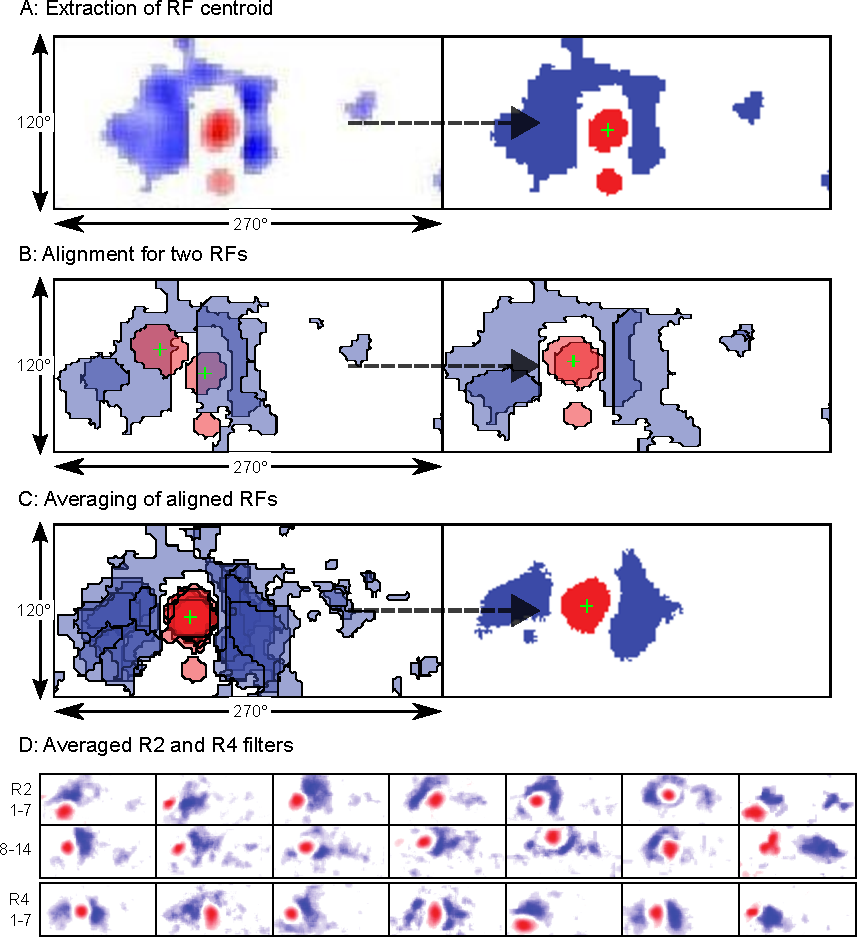
\includegraphics{figures/avkernels}
\caption{The algorithm for obtaining average RFs.}{
A: The raw image (left) is thresholded so as to give excitatory and inhibitory regions of uniform intensity (right).
The `centre' is then calculated as the centroid of the largest excitatory region (+).
B: Aligning two RFs.
The new centre is taken as the average of the centre of both RFs and the RFs are then shifted so that the centres are aligned.
C: Averaging the RFs for this glomerulus over all flies ($N=7$), following alignment.
Note that this the left-hemispheric version; the right-hemispheric version is its mirror.
Data are all for R4d glomerulus 1 neurons.}
\label{fig:avkernels}
\end{figure}


\subsection{Replication of behavioural experiments}
\label{sec:methods:replication}
The equation for describing the bar fixation mechanism shown in Figure~\ref{fig:recap}C is as follows:
$$
\phi_\mathrm{turn} = \frac{\mathrm{gain}\cdot \pi}{4}\left( \sum\limits_{K\in \mathbf{G}_\mathrm{left}}\max(0,A(I,K,0\degree)) - \sum\limits_{K\in \mathbf{G}_\mathrm{right}}\max(0,A(I,K,0\degree)) \right)
$$
where $I$ is the view of the bar from the agent's current location and $\mathbf{G}_\mathrm{left}$ and $\mathbf{G}_\mathrm{right}$ are the sets of left- and right-hemispheric filters. `Gain' is a parameter to control the gain of the system, and here was set to 2.

For the pattern recognition tasks (see Figure~\ref{fig:pattern}), the difference in activation is calculated as follows:
$$
D(I) = \sqrt{\frac{\sum\limits_{K\in \mathbf{G}}(A(I,K,0\degree)-A(I,K,90\degree))^2}{|\mathbf{G}|}}
$$
where $\mathbf{G}$ is the set of R2 filters, $I$ is the current pattern pair and $A(\cdot,\cdot,\cdot)$ is the activation of the kernel to the pattern, as described in Equation~\ref{eq:act}.

\subsection{Neural networks}
\label{sec:methods:neuralnetworks}
The neural networks were executed using the \texttt{Netlab} toolbox for \Matlab.
All networks were two-layer feedforward networks, with 10 hidden units and a linear activation function for the output units.
There were 100 training cycles and optimisation was performed with the scaled conjugate gradient method.

\subsubsection{Stimuli}
\label{sec:methods:stimuli}
The stimuli used to train the networks were trained were a series of black `blobs' on a white background.
The blobs were based on ellipses with a fixed ratio between the lengths of the major and minor axes ($2:1$), with the radii modified with complex waves:
$$
r(\theta) \le \left(\frac{\cos^2 \theta}{2} + \frac{\sin^2 \theta}{a} \right)^{-1} + W(\theta), \theta \in \{0, 2\pi\}
$$
where $a$ is the length of the major axis and $W(\theta)$ is a complex wave defined as:
$$
W(\theta) = \sum_{i=1}^n W_i(\theta) = \sum_{i=1}^n A_i \sin f_i (\theta+\phi_i) 
$$
where $A_i$, $f_i$ and $\phi_i$ describe the maximum amplitude, frequency and phase shift of the wave $W_i(\theta)$, respectively.
This method for generating stimuli allows for a substantial degree of random variation between the stimuli, while not producing shapes that are so irregular as to be unlearnable by a neural network.\todo{insertion}

In these experiments, $A_i$, $f_i$ and $\phi_i$ were randomly generated and $n=2$.
$A_i$ was a random value from 0 to 1, $f_i$ were random integers from 1 to 30 and $\phi_i$ was a random value from 0 to $2\pi$.
\begin{comment}
        nvar = 1000;
        nwave = 2;
        maxfreq = 30;
        maxamp = 1;
\end{comment}

The blobs were first generated, according to the above equation, as an image of $120\times 270$ pixels.
For the `raw view' stimuli, these images were resized, using \Matlab's \texttt{imresize} function, to $2\times 14$ pixels, thus giving the same number of inputs as there are R2 filters ($n=28$).

\begin{comment}
\subsubsection*{Grading performance of neural networks}
The performance of neural networks was graded by calculating the \ac{rms} difference between the matrix of true values for the parameters with the network's output:
$$
E(\mathbf{y},\mathbf{t}) = \sqrt{\frac{\sum\limits_{i=1}^{n} (\mathbf{y}_i-\mathbf{t}_i)^2}{n}}
$$
where $E(\mathbf{y},\mathbf{t})$ is the mean error score, computed from the vector of outputs given by the network, $\mathbf{y}$, and the vector of true values, $\mathbf{t}$.
Hence, for a network that computed the values of all parameters accurately, a graph of the network's output \emph{vs.} the true values would give the line $y=x$ and an error score of 0 over the whole range of values.
\end{comment}


\bibliographystyle{plos2009}
\bibliography{library}

\begin{figure}
\centering
\includegraphics{figures/recap}
\caption{Simulation of fly pattern discrimination paradigm. A standard experimental paradigm for testing the pattern discrimination abilities of \emph{Drosophila} \protect\cite{Ernst1999} can be replicated in simulation.
A: A diagram showing Buridan's paradigm \protect\cite{Bulthoff1982,Gotz1980}. If a fly is placed in an arena between two large vertical bars, it will walk back and forth until exhaustion.
B and C: The mean output of R2 (blue) and R4d (green) filters, from different headings, to bars of different widths. The blue crosses in A indicate the points from which bars B and C are being viewed.
D: The fly is held tethered in a drum. As the fly attempts to rotate about its yaw-axis, the drum rotates in the opposite direction, thus allowing the fly to select the portion of the pattern in view.
By monitoring the fly's heading, one can surmise whether there is a spontaneous preference for one of the patterns.
Whether the fly can learn to head towards one pattern is tested by adding a laser that punishes the fly for facing one of the patterns.
Shown inside the drum are the visual \acp{RF} for one pair of left- and right-hemispheric glomeruli.
E and F: The \ac{rms} difference in output for R2 (blue) and R4d (green) neurons as the pattern is rotated.
The reference activities are the \ac{RF} outputs when the simulated flies are at 0\degree.
Patterns with a greater difference in activity at 0\degree\ \emph{vs} 90\degree\ should be more discriminable by flies.
For two pairs of patterns we show that there is a much smaller difference in output when the triangles are aligned about the vertical centre of mass (E) than not (F).
This mirrors real flies' performance on this task \protect\cite{Ernst1999}.}
\label{fig:recap}
\end{figure}

\begin{figure}
\vspace{-1cm}
\centering
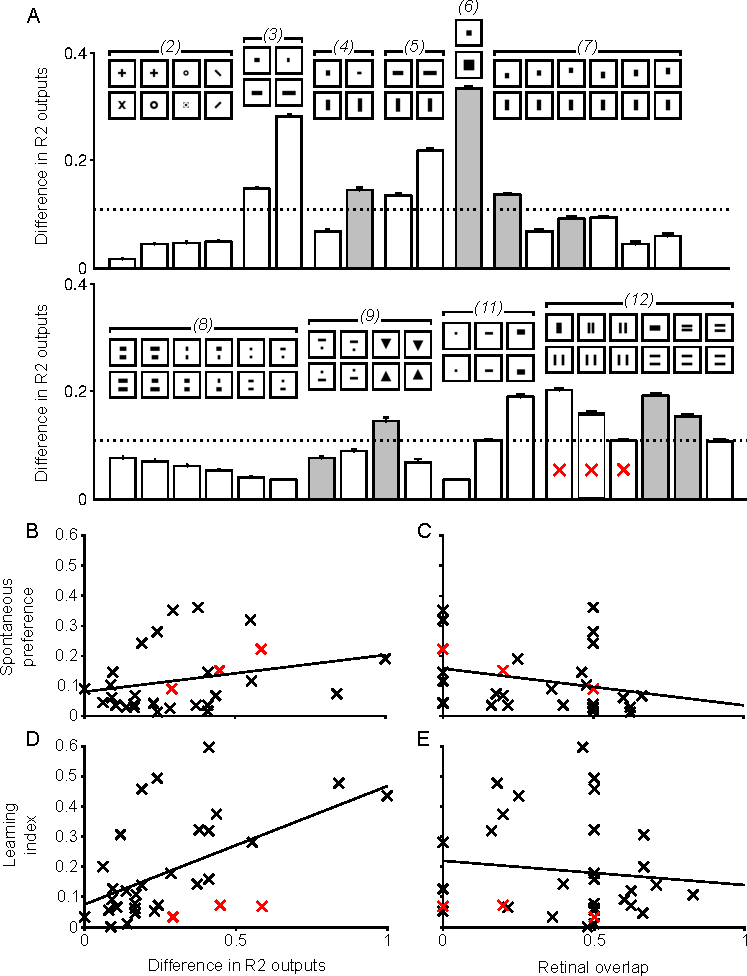
\includegraphics{figures/pattern}
\caption{[NB: I haven't put in the pattern pairs yet, but this should give an idea of the layout.]
Outputs of simulated R2 cells for published pattern pairs. Whether a pattern pair is discriminable by flies can be predicted partly on the basis of the difference in R2 activity.
The patterns tested here are drawn from \protect\cite{Ernst1999} and are grouped together according to the figures in which they appear in that work.
The corresponding figure numbers are shown in parentheses.
All patterns for which the significance of `learning preference' ($\overline{\mathrm{DCP}}$) was given are included.
Grey bars indicate that the $\overline{\mathrm{DCP}}$ for the pattern was significant ($p<.05$).
A higher score indicates a greater \ac{rms} difference in R2 activity and thus that the pattern was more discriminable by the simulation.
In general, within these groups, the patterns where there was a significant learned preference (in \protect\cite{Ernst1999}) have a greater difference in activity.
Performance on more `horizontal' patterns (e.g. \emph{(3)} and the final three patterns in \emph{(12)}) was poor in the behavioural experiments, but better in simulation.
This is perhaps due to the horizontal motion of the patterns in training, as noted in \protect\cite{Ernst1999}.
At the bottom are shown scatter plots of R2 difference (the `RF Model') and retinal overlap (the `Retinotopic Model') \emph{vs} learning index ($\overline{\mathrm{DCP}}$) shown in Ernst and Heisenberg \protect\cite{Ernst1999}.
The correlation for the RF Model was found to be significant (Spearman's rank, $n=34, \rho=.615, p<.005$), but not for the Retinotopic Model ($n=34, \rho= -0.215, p=\mathrm{n.s.}$).
}
\label{fig:pattern}
\end{figure}

\begin{figure}
\vspace{-3cm}
\centering
\includegraphics{figures/simdiffpatts}
\caption{
[PRG]
R2 cells do not encode detailed shape information.
A--C. The discriminability of pattern pairs can vary greatly independently of the apparent difference between visual stimuli. A. A pattern pair made up of a triangle and its inverse with both triangles aligned to their lowest points. B. The same triangles, but this time aligned by their centres of mass, make another pattern pair. C. The difference in activation between 0\degree\ and 90\degree\ for all R2 RF filters for the triangles from A (open bars)and B (closed bars). The mean activation difference is greater for the triangles in A over B. The red square marks the output of the ring neuron RF shown in A,B. 
D--F. We can also generate shapes that appear similar yet produce a large mean difference in RF activation (D) or appear different and produce similar RF activations (E). The stimuli here are `blobs' of the form described in Methods. An optimisation was performed in Matlab (\texttt{fminsearch} function) to minimise the ratio of blob difference to difference in activation (D) or its inverse (E). Pairs of stimuli are shown in grey and green whereas in the simulation both are black.
F. The corresponding activations of separate (left-hemispheric) R2 glomeruli are shown at the bottom. Two similar patterns give a mean difference in activity of 11.0\%. Two very different patterns give a mean difference in activity of 5.10\%.
}

\label{fig:simdiffpatts}
\end{figure}
%\begin{figure}
\centering
\includegraphics{figures/bar}
\caption{R2 and R4d neurons show patterns of activation that match simple orientation behaviours.
A: The responses of left- and right-hemispheric R2 and R4d \acp{RF} to black vertical bars of different widths.
R2 neurons respond maximally to the inside edges of the three largest bars, which is where flies head when presented with wide vertical bars \protect\cite{Osorio1990}.
For the R4d neurons, peaks in activation occur at the bar's centre and also at roughly $\pm 90\degree$ to it, where saccade amplitude will be greatest for an agent performing bar fixation.
B and C: Outputs of the \acp{RF} can be used to drive bar homing, as shown by the vector plot in B.
The algorithm used to generate these data is shown in C.
D: The \ac{RF} outputs also provide information about vertical bar-like objects in a natural scene.
The proportion of \acp{RF} whose activity level was greater than one SD from the mean is shown (blue: R2 neurons; green: R4d neurons).
The natural image was converted to greyscale before processing.
(Photograph: University of Sussex campus, UK, taken with a Sony Bloggie\texttrademark\ panoramic camera.)}

\label{fig:bar}
\end{figure}

\begin{figure}
\centering
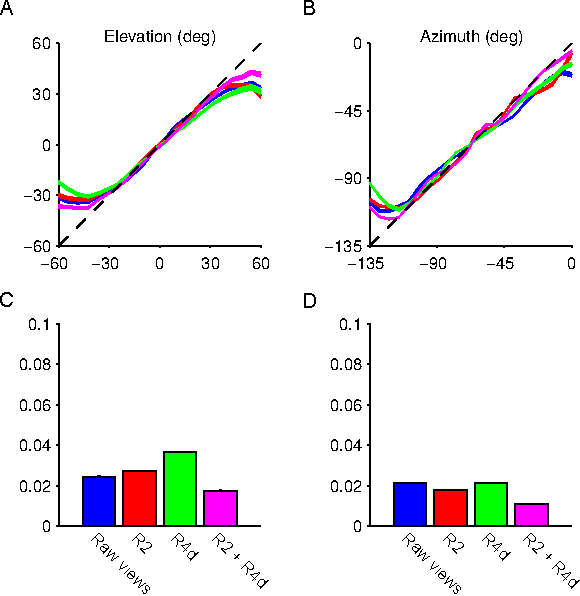
\includegraphics{drosopattern/elaz}
\thesiscaption{How much positional information is preserved in the R2 population code?}{
Neural networks were trained to estimate the elevation and azimuth of randomly generated `blob' stimuli ($N=10,000$)  from raw views ($N=36$~pixels; blue), R2 neurons ($N=28$; red), R4d neurons ($N=14$; green) or R2 and R4 neurons ($N=42$; magenta). For each visual input a network was trained 100 times and average performance with blobs that were not part of the training set was taken.
A and B: Plots of elevation and azimuth of the test visual stimuli \emph{vs} the mean network output ($N=100$). The dashed line indicates ideal performance (i.e. $y=x$) and the thickness of the lines at each point shows standard error.
The possible values of elevation and azimuth were constrained by the size of the fruitfly visual field (approx. $120\degree \times 270\degree$). Within this range there were 22 possible values.
C and D: Average network performance (mean square error) for networks trained to recover elevation (C) or azimuth (D) and for each type of visual input (colour code as above). Standard error is shown, but is very small.
}
\label{fig:drosopattern:elaz}
\end{figure}

\begin{figure}
\centering
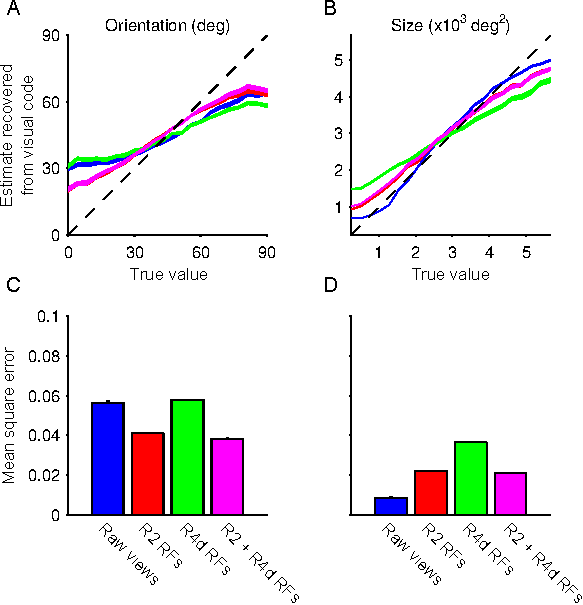
\includegraphics{figures/orsi}
\caption{How much shape information is preserved in the R2 population code?
Neural networks were trained to estimate the orientation and size of randomly generated 'blob' stimuli ($N=1000$) from different visual encodings (details same as for Figure~\ref{fig:elaz}).
A and B: Network performance in recovering stimulus orientation and size. Orientation was constrained between 0\degree\ and 90\degree, to avoid the problem of aliasing, and varied with 22 levels (conventions as in Figure~\ref{fig:elaz}).
C and D: Average network performance (mean square error) for networks trained to recover orientation (C) or size (D) and for each type of visual input (colour code as previously). Standard error is shown, but is very small.
}
\label{fig:orsi}
\end{figure}

\begin{figure}
\centering
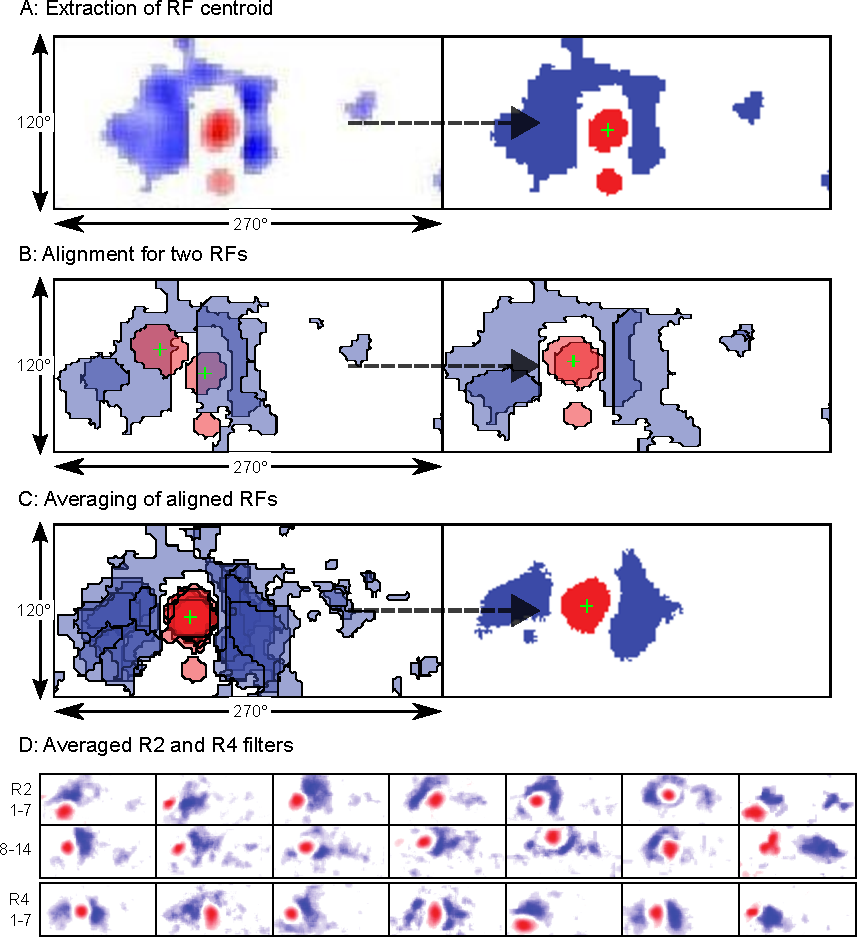
\includegraphics{figures/avkernels}
\caption{The algorithm for obtaining average RFs.}{
A: The raw image (left) is thresholded so as to give excitatory and inhibitory regions of uniform intensity (right).
The `centre' is then calculated as the centroid of the largest excitatory region (+).
B: Aligning two RFs.
The new centre is taken as the average of the centre of both RFs and the RFs are then shifted so that the centres are aligned.
C: Averaging the RFs for this glomerulus over all flies ($N=7$), following alignment.
Note that this the left-hemispheric version; the right-hemispheric version is its mirror.
Data are all for R4d glomerulus 1 neurons.}
\label{fig:avkernels}
\end{figure}


\end{document}
